%FOR PDFLATEX USE ONLY
\documentclass[a4paper,12pt]{article}

\usepackage{amssymb,amsmath} %math symbols

\usepackage[margin=2cm]{geometry} %paper geometry

\usepackage[utf8]{inputenc} %allows unicode (including russian) source file
\usepackage[russian]{babel} %docment in russian-style
\usepackage[utf8]{inputenc}
%\usepackage[unicode]{hyperref} %links inside of the text
\usepackage[pdftex]{graphicx} %includegraphics pictures
\usepackage{cmlgc} %bold text

\usepackage{array} %arrays

%\usepackage{wrapfig}
%\usepackage{array}
%\usepackage{lipsum}
%\usepackage{esvect}
%\usepackage{hyperref}

\usepackage{subfig}
%\usepackage{calc}
%\usepackage{pgfplots,tikz,circuitikz}
%\usepackage{tkz-euclide}
\usepackage{booktabs}
\usepackage{multirow}

\usepackage{wrapfig}

\begin{document}

\begin{center}
  \LARGE{Работа 4.7.1}\\[0.2cm]
  \LARGE{Двойное лучепреломление}\\[0.2cm]
  \large{Малиновский Владимир}\\[0.2cm]
  \normalsize{\texttt{galqiwi@galqiwi.ru}}
\end{center}

\textbf{Цель работы}: изучение зависимости показателя преломления необыкновенной волны от направления в двоякопреломляющем кристалле; определение главных показателей преломления $n_o$ -- обыкновенной и $n_e$ -- необыкновенной волны в кристалле; наблюдение эффекта полного внутреннего отражения

\textbf{В работе используются}: лазерная указка, вращающийся сотолик с неподвижным лимбом, призма из исландского шпата, поляроид.
\section*{Описание работы}

\section*{Теория}
\subsection*{Плоские волны в кристаллах}
\begin{equation}
\text{rot} \vec{H} = \dfrac{1}{c}\dfrac{\partial \vec{D}}{\partial t}, \text{rot} \vec{E} = -\dfrac{1}{c}\dfrac{\partial \vec{B}}{\partial t}
\end{equation}
Если среды прозрачны и однородны то в них распорстраняются волны:
\begin{equation}
\vec E = \vec{E}_0 e^{i(\omega t - \vec{k}\vec{r})}, \vec{H} = \vec{H}_0e^{i(\omega t - \vec{k}\vec{r})}
\end{equation}
Введем единичный вектор нормали к скорости распространения волны $\vec{N}$ и направим его вдоль скорости, тогда
\begin{equation}
\vec{D} = -\dfrac{c}{v}\left[\vec{N}, \vec{H}\right], \vec{B} = \dfrac{c}{v}\left[  \vec{N}, \vec{E}\right]
\end{equation}
\subsection*{Оптические одноосные кристаллы}
Введем \textit{тензор диэлектрической проницаемости} $\varepsilon$ ($\vec{D} = \varepsilon \vec{E}$). Все его значения описываются эллипсоидом инерции. 

В кристаллах этот эллипсоид --- эллипсоид вращения. В них оптическая ось --- ось вращения эллипсоида. В них принято обозначать $\varepsilon_{\parallel} = \varepsilon_z, \varepsilon_{\perp} = \varepsilon_x = \varepsilon_y$

\begin{equation}
\vec{D}_{\parallel} = \varepsilon_{\parallel} \vec{E}_{\parallel},\vec{D}_{\perp} = \varepsilon_{\perp} \vec{E}_{\perp} 
\end{equation}

Можно показать, что угол $\theta$ между волновой нормалью и осью вращения эллипсоида при разделении $\vec{D}$ на $\vec{D}_e$ --- лежащая в главном сечении и $\vec{D}_o$ --- нормальная составляющая такой, что
\begin{equation}
\sin \theta = \dfrac{D_{e\parallel}}{D_e}, \cos \theta = \dfrac{D_{e\perp}}{D_e}
\end{equation}
\begin{equation}
n = \dfrac{1}{\sin A}\sqrt{\sin^2 \varphi_1 + \sin^2 \varphi_2 + 2 \sin \varphi_1 \sin \varphi_2 \cos A}
\end{equation}
Из этого, если $n_o - n_e \ll n_o$ и $n_e$, то 
\begin{equation}
n(\theta) \approx n_e + (n_o - n_e) \cos^2 \theta
\end{equation}
%\newpage
\subsection*{Двойное лучепреломление в призме исландского шпата}
\begin{wrapfigure}{r}{0.3\textwidth}
  \begin{center}
    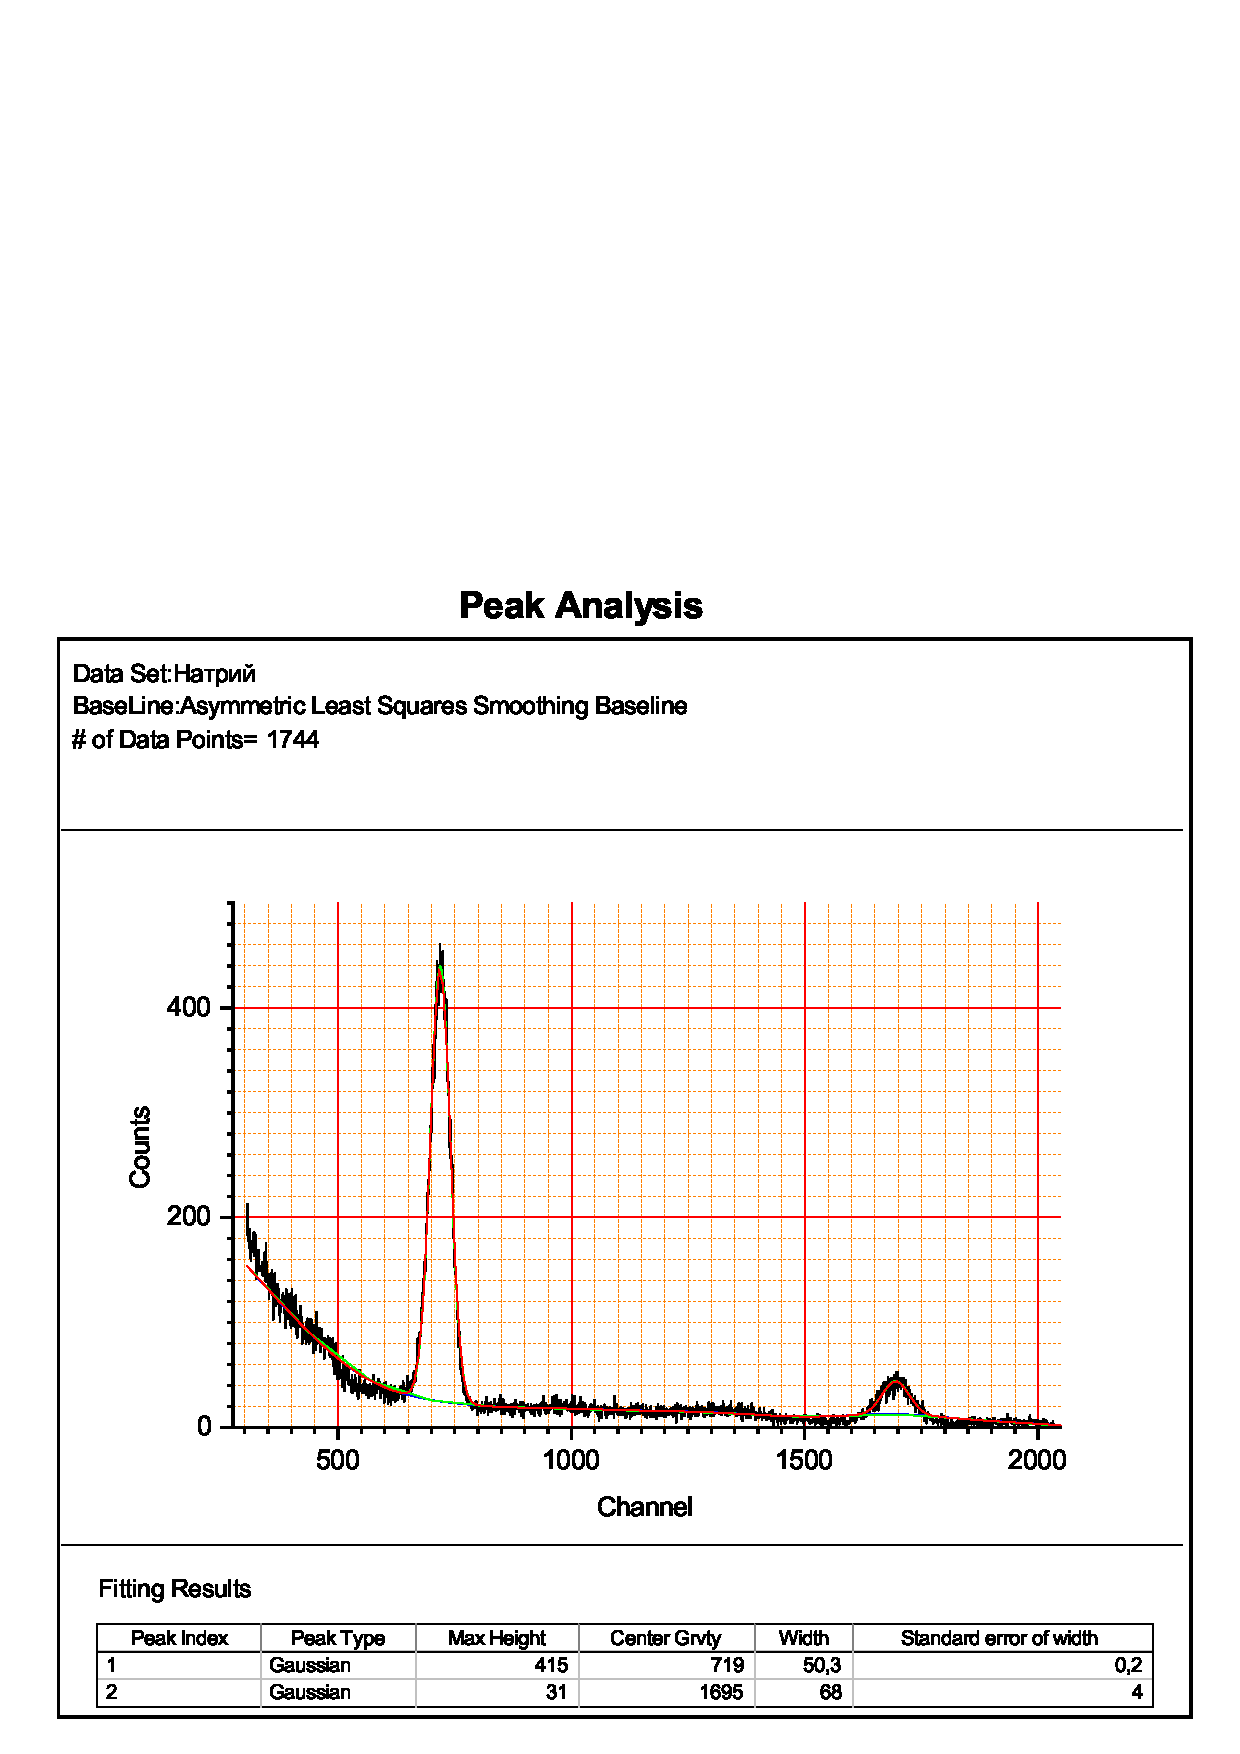
\includegraphics[width = 0.2\textwidth]{1.png}
  \end{center}
  \caption{Ход луча в призме}
\end{wrapfigure}
При таком ходе луча и расположении призмы у нас повторяется ситуация из предыдущего параграфа теории. Тогда, можно посчитать показатель преломления изотропной среды по формуле 
\begin{equation}
n = \dfrac{\sin\left(\dfrac{\psi_m + A}{2}\right)}{\sin \left(\dfrac{A}{2}\right)}
\end{equation}
Здесь $\psi_m$  --- минимальный угол, на который призма преломляет луч.
Если призма неизотропна, то этой формулой, строго говоря, можно воспользоваться только для обыкновенной волны, которая, как это было показано ранее, распространяется так же, как и в изотропной среде. 
\section*{Экспериментальная установка}

\begin{figure}[h]
\begin{center}
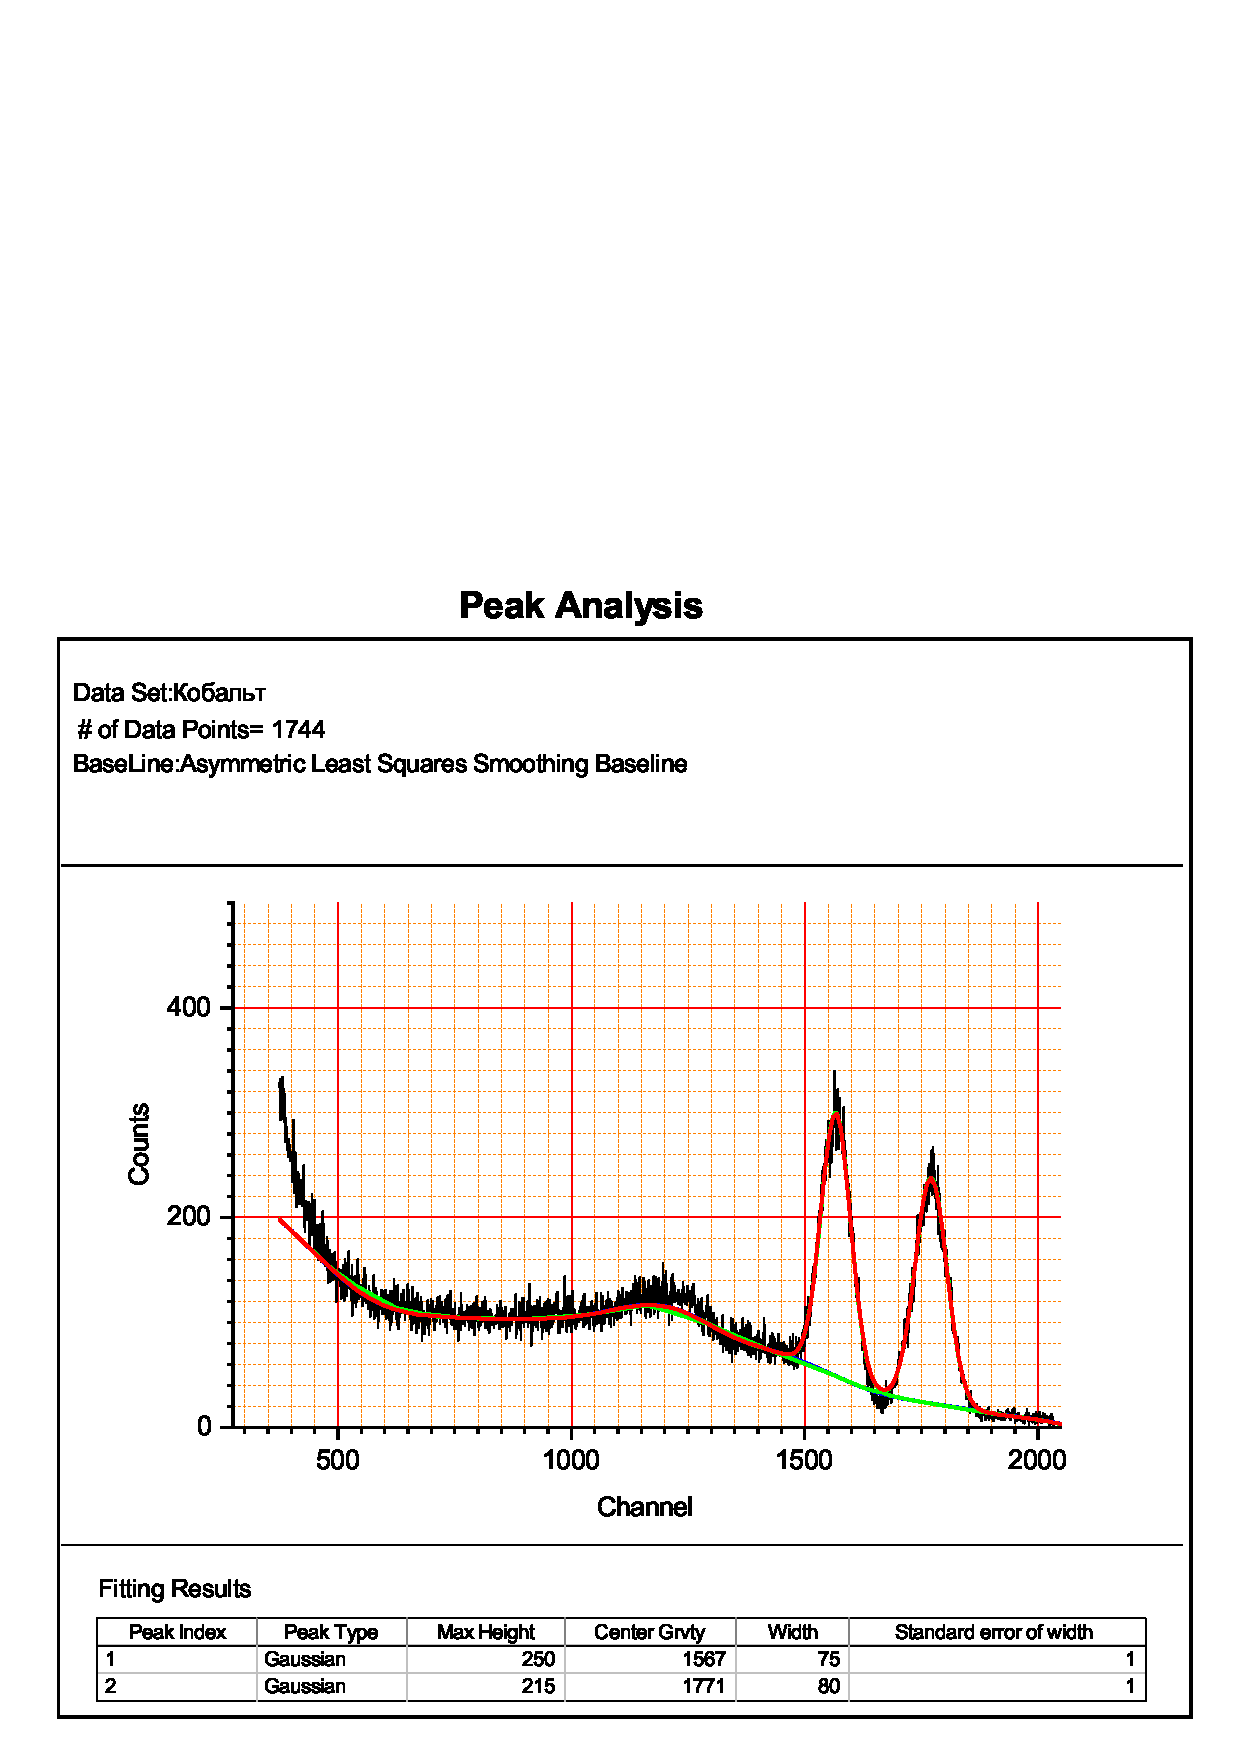
\includegraphics[width = 0.7\textwidth]{2.png}
\caption{Экспериментальная установка}
\end{center}
\end{figure}
\begin{equation}
\varphi_2 = A + \psi - \varphi_1
\end{equation}

\section*{Результаты и обработка}
\subsection*{1}
Отъюстируем установку. Для этого отцентруем экран по лучу лазера, то есть убедимся, что луч проходит под отметками $0$ и $180$.
\subsection*{2}
Отметим два положения риски, при которых луч, отраженный от входной и рабочей грани, попадает обратно на отметку $0$. Получим значения
\[\varphi_0 = (296\pm0.5)^\circ,\,\varphi_1 = (154\pm0.5)^\circ.\]
Из геометрии получим формулу для $A$
\[A=180^\circ-(\varphi_0-\varphi_1) = (38\pm1)^\circ.\]
\subsection*{3-4}
Определим разрешенное положение поляризатора --- для этого направим его на стол и добьемся минимальной интенсивности проходящего света.\\
Поставим поляризатор с известным разрешенным направлением перед призмой. Один из лучей, проходящих через линзу, потеряет в интенсивности. Это будет необыкновенный луч.

\begin{center}
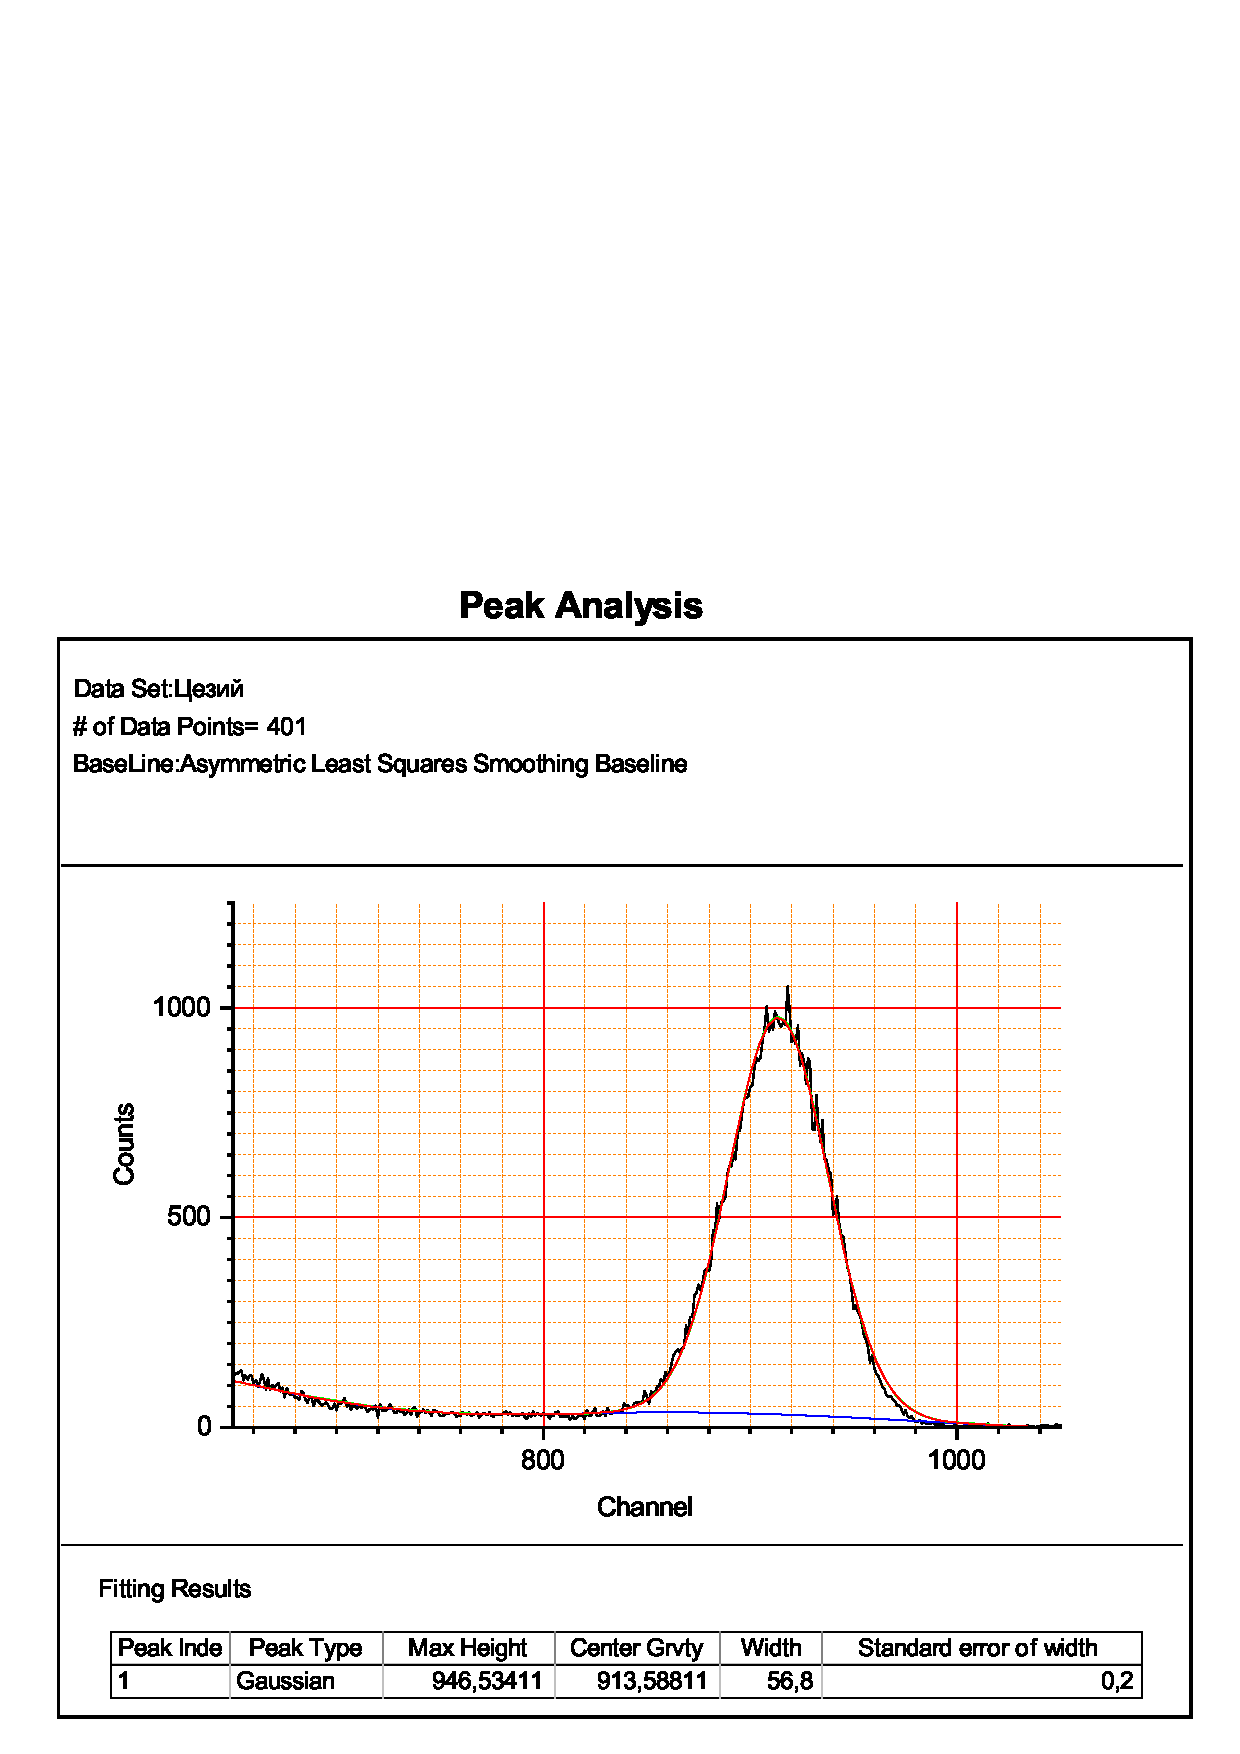
\includegraphics[width=0.95\textwidth]{3.png}
необыкновенный луч снизу
\end{center}

\subsection*{5-7}
Начнем вращать столик, измерим пары значений $2\varphi_1$ и $180^\circ+\psi$. Из формулы (6) получим значение $n_o$ коэффициент преломления обычной волны и $n_e$ необыкновенной. 

\begin{center}
\includegraphics[width=0.95\textwidth]{4.png}
\end{center}

\begin{center}
\begin{tabular}{|c|c|c|c|c|c|c|}\hline
$2 \phi_1$&$180+\psi_e$&$180+\psi_o$&$n_e$&$\Delta n_e$&$n_o$&$\Delta n_o$\\\hline
$0.0$&$207.0$&$-$&$1.472$&$0.007$&$-$&$-$\\\hline
$4.0$&$205.0$&$222.0$&$1.466$&$0.007$&$1.634$&$0.005$\\\hline
$10.0$&$203.0$&$216.0$&$1.461$&$0.008$&$1.630$&$0.006$\\\hline
$15.0$&$202.0$&$214.0$&$1.462$&$0.009$&$1.638$&$0.007$\\\hline
$20.0$&$202.0$&$212.0$&$1.477$&$0.009$&$1.638$&$0.007$\\\hline
$25.0$&$201.0$&$210.0$&$1.47$&$0.01$&$1.630$&$0.008$\\\hline
$30.0$&$201.0$&$209.0$&$1.48$&$0.01$&$1.632$&$0.009$\\\hline
$35.0$&$200.0$&$208.0$&$1.471$&$0.011$&$1.629$&$0.009$\\\hline
$40.0$&$200.0$&$208.0$&$1.478$&$0.011$&$1.64$&$0.01$\\\hline
$45.0$&$200.0$&$207.0$&$1.483$&$0.011$&$1.63$&$0.01$\\\hline
$50.0$&$200.0$&$207.0$&$1.487$&$0.011$&$1.640$&$0.011$\\\hline
$55.0$&$200.0$&$207.0$&$1.489$&$0.012$&$1.646$&$0.011$\\\hline
$60.0$&$200.0$&$207.0$&$1.489$&$0.012$&$1.649$&$0.011$\\\hline
$65.0$&$200.0$&$207.0$&$1.487$&$0.012$&$1.650$&$0.011$\\\hline
$70.0$&$200.0$&$207.0$&$1.484$&$0.012$&$1.649$&$0.012$\\\hline
$75.0$&$201.0$&$207.0$&$1.503$&$0.012$&$1.646$&$0.012$\\\hline
$80.0$&$201.0$&$207.0$&$1.497$&$0.012$&$1.640$&$0.012$\\\hline
$85.0$&$202.0$&$207.0$&$1.512$&$0.012$&$1.633$&$0.012$\\\hline
$90.0$&$202.0$&$208.0$&$1.502$&$0.012$&$1.647$&$0.012$\\\hline
$95.0$&$203.0$&$208.0$&$1.514$&$0.012$&$1.635$&$0.012$\\\hline
$100.0$&$203.0$&$209.0$&$1.501$&$0.012$&$1.645$&$0.012$\\\hline
$105.0$&$204.0$&$210.0$&$1.509$&$0.012$&$1.652$&$0.012$\\\hline
$110.0$&$205.0$&$210.0$&$1.515$&$0.012$&$1.634$&$0.012$\\\hline
$115.0$&$206.0$&$211.0$&$1.519$&$0.012$&$1.637$&$0.012$\\\hline
$120.0$&$207.0$&$212.0$&$1.521$&$0.012$&$1.638$&$0.012$\\\hline
$125.0$&$208.0$&$213.0$&$1.520$&$0.012$&$1.637$&$0.012$\\\hline
$130.0$&$210.0$&$215.0$&$1.540$&$0.012$&$1.656$&$0.012$\\\hline
$135.0$&$211.0$&$216.0$&$1.534$&$0.012$&$1.649$&$0.012$\\\hline
$140.0$&$212.0$&$217.0$&$1.526$&$0.012$&$1.640$&$0.012$\\\hline
$145.0$&$214.0$&$219.0$&$1.538$&$0.012$&$1.651$&$0.012$\\\hline
$150.0$&$215.0$&$220.0$&$1.525$&$0.012$&$1.637$&$0.012$\\\hline
$155.0$&$217.0$&$222.0$&$1.531$&$0.012$&$1.642$&$0.012$\\\hline
$160.0$&$219.0$&$224.0$&$1.533$&$0.012$&$1.645$&$0.012$\\\hline
$165.0$&$221.0$&$226.0$&$1.533$&$0.012$&$1.644$&$0.012$\\\hline
$170.0$&$224.0$&$228.0$&$1.552$&$0.012$&$1.641$&$0.012$\\\hline
$175.0$&$227.0$&$232.0$&$1.568$&$0.012$&$1.679$&$0.013$\\\hline
\end{tabular}\\~\\
$\Delta 2 \phi_1=0.5\,\text{}, \Delta 180+\psi_e=0.5\,\text{}, \Delta 180+\psi_o=0.5\,\text{}$
\end{center}



\begin{center}
\includegraphics[width=0.95\textwidth]{down_up.png}
\end{center}

Из графика $n_e$ получается
\[n_e = (1.47\pm0.01),\,n_o = (1.64\pm0.01).\]
Из графика $n_0$ получается
\[n_0 = (1.64\pm0.01).\]

\begin{center}
\includegraphics[width=0.95\textwidth]{down_up_1.png}
Демонстрация того, что значениe $n_o$ получается одинаковым независимо от метода получения.
\end{center}

\subsection*{8}
Найдем минимальные значения $\psi$. Для этого заметим, что при минимальном значении производная $\frac{\delta \psi}{\delta \varphi_1}$ становится равна $0$. Этот факт позволяет точно получить значение $\psi_m$. Вокруг минимального значения начнем периодично менять $\varphi_1$. Область, в которой незаметно движение лазерного пятна -- это область, в которой достигается минимальное значение $\psi$.
\[\psi_{om} = (27.0\pm0.5)^\circ,\,\psi_{em} = (27.0\pm0.5)^\circ.\]
Из этого получается значение $n$
\[n_o = (1.49\pm0.02),\,n_e = (1.65\pm0.02).\]
\subsection*{9}
Найдем углы падения, соответсвующие полному внутреннему отражению. Для этого найдем критические значения $\varphi_{1e}$ и $\varphi_{1o}$, при которых необыкновенный и обыкновенный луч соответственно проходят через полное отражение от второй грани призмы
\[\varphi_{1o} = (0.0\pm0.3)^\circ,\,\varphi_{1o} = (-5.0\pm0.3)^\circ.\]
Принимая $\varphi_2=90^\circ$, найдем значение $n_o$ и $n_e$ из (6)
\[n = \frac{1}{\sin A}\sqrt{\sin^2\varphi_1 + 1 + 2 \sin\varphi_1\cos A}.\]
Из формулы выше получаем
\[n_e = (1.41\pm0.04),\,n_o = (1.62\pm0.03).\]
Табличные значения из лабника
\[n_e = 1.485,\,n_o = 1.655.\]

\section*{Вывод}
С помощью трех методов мы измерили коэффициент преломления необыкновенной и обыкновенной волны у исландского шпата. Данные совпали с табличными с точностью до 2 цифры после запятой.
\end{document}








\lipsum[1-4]
\begin{wrapfigure}{R}{5cm}
\centering
\includegraphics[width=0.20\textwidth]{rd.png}
\caption{1}
\end{wrapfigure}
\lipsum[1-6]


\begin{figure}[h]
\begin{center}$
\begin{array}{cccc}
\includegraphics[width=0.20\textwidth]{rd.png}&
\includegraphics[width=0.20\textwidth]{rd.png}&
\includegraphics[width=0.20\textwidth]{rd.png}&
\includegraphics[width=0.20\textwidth]{rd.png}\\
(1) & (2) & (3) & (4)
\end{array}$
\end{center}
\end{figure}
